\let\negmedspace\undefined
\let\negthickspace\undefined
\documentclass[journal]{IEEEtran}
\usepackage[a5paper, margin=10mm, onecolumn]{geometry}
\usepackage{tfrupee}

\setlength{\headheight}{1cm}
\setlength{\headsep}{0mm}

\usepackage{gvv-book}
\usepackage{cite}
\usepackage{amsmath,amssymb,amsfonts,amsthm}
\usepackage{algorithmic}
\usepackage{graphicx}
\usepackage{textcomp}
\usepackage{xcolor}
\usepackage{txfonts}
\usepackage{listings}
\usepackage{enumitem}
\usepackage{mathtools}
\usepackage{gensymb}
\usepackage{comment}
\usepackage[breaklinks=true]{hyperref}
\usepackage{tkz-euclide} 
\usepackage{listings}
\usepackage{gvv}                                        
\usepackage{tikz}
\def\inputGnumericTable{}                                 
\usepackage[latin1]{inputenc}                                
\usepackage{color}                                            
\usepackage{array}                                            
\usepackage{longtable}                                       
\usepackage{calc}                                             
\usepackage{multirow}                                         
\usepackage{hhline}                                           
\usepackage{ifthen}                                           
\usepackage{lscape}
\begin{document}

\bibliographystyle{IEEEtran}

\title{1.9.5}
\author{EE25BTECH11016 - Taraka Abhinav}
{\let\newpage\relax\maketitle}

\renewcommand{\thefigure}{\theenumi}
\renewcommand{\thetable}{\theenumi}
\setlength{\intextsep}{10pt}

\numberwithin{figure}{enumi}
\renewcommand{\thetable}{\theenumi}

\textbf{Question}:\\
Find the distance between the points $\brak{0,2\sqrt{5}}$ and $\brak{-2\sqrt{5},\,0}$. \hfill $\brak{10,2021}$
\\

\solution \\

\begin{table}[h!]    
  \centering
  \begin{tabular}{|c|c|}
  \hline
  Symbol & Description \\
  \hline
  $\vec{A}$ & Point $\brak{0,2\sqrt{5}}$ \\
  $\vec{B}$ & Point $\brak{-2\sqrt{5},0}$ \\
  $d$ & Distance between $A$ and $B$ \\
  \hline
  \end{tabular}
  \caption{Variables Used}
  \label{tab10.5.8.2}
\end{table}

\begin{align}
\vec{A} &= \myvec{0\\2\sqrt{5}}, \quad 
\vec{B} = \myvec{-2\sqrt{5}\\0}
\end{align}

The distance between two points is given by
\begin{align}
d &= \norm{\vec{A}-\vec{B}}
\end{align}

Substituting values,
\begin{align}
d &= \norm{\myvec{0\\2\sqrt{5}}-\myvec{-2\sqrt{5}\\0}} \\ 
  &= \norm{\myvec{2\sqrt{5}\\2\sqrt{5}}} \\ 
  &= \sqrt{(2\sqrt{5})^2 + (2\sqrt{5})^2}
\end{align}

Simplifying,
\begin{align}
d &= \sqrt{20 + 20} \\
  &= \sqrt{40} \\
  &= 2\sqrt{10}
\end{align}

\begin{align}
\implies d = \boxed{2\sqrt{10}}
\end{align}

\begin{figure}
    \centering
    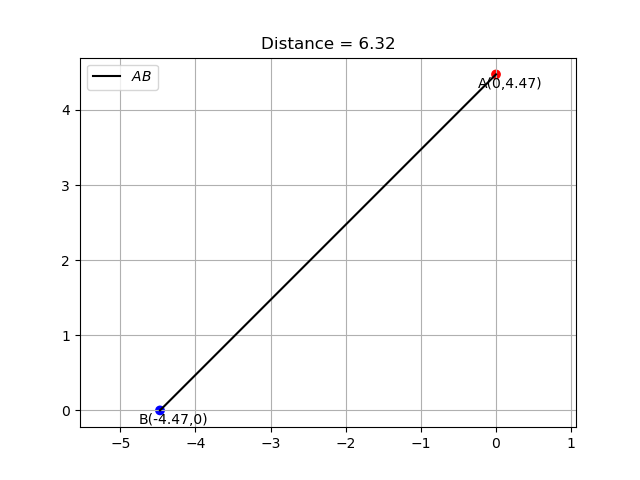
\includegraphics[width=0.8\columnwidth]{figs/Figure_1.png}
    \label{fig:placeholder}
\end{figure}

\end{document}
